\chapter{Macrosegregation with solidification shrinkage}
%\chaptermark{Nonlinear Temperature Solver}
\begin{nolinkcolors} 
\minitoc
\end{nolinkcolors}
\newpage

% ======================
\section{Solidification shrinkage}
% ======================

Solidification shrinkage is, by definition, the effect of relative density change between the liquid and solid phases.
In general, it results in a progressive volume change during solidification, until the phase change has finished. 
The four stages in \cref{fig:real_ingot_stage_a,fig:real_ingot_stage_c,fig:real_ingot_stage_b,fig:real_ingot_stage_d} depict the volume change with 
respect to solidification time.
First, at the level of the first solid crust, near the local solidus temperature, the solid forms with a density greater than 
the liquid's. The subsequent volume decrease creates voids with a negative pressure, forcing the fluid to be sucked in the direction of the volume change 
(cf. \cref{fig:real_ingot_stage_b}). As a direct result of the inward feeding flow, the ingot surface
tends to gradually deform in the feeding direction, forming the so-called \emph{shrinkage pipe}. Since the mass of the alloy and its 
chemical species is conserved, a density difference between the phases ($\rhol < \rhos \implies \frac{\rhol}{\rhos}<1$) eventually leads 
to a different overall volume ($V^s<V^l$) once solidification is complete, as confirm the following equations:
%------------
\begin{subequations}
\begin{align}
& \rhol V^l = \rhos V^s  \\ 
& V^s = \frac{\rhol}{\rhos} V^l
\end{align}
\end{subequations}
%------------
Solidification shrinkage is not the only factor responsible for volume decrease. Thermal shrinkage in both solid and liquid phases, as well 
as solutal shrinkage in the liquid phase are also common causes in a casting process. However, thermal shrinkage is very important to apprehend
as temperature decrease in steel casting usually exceeds a \SI{1000}{\udegC}, causing substantial density variations. 
%Henceforth, we will focus on shrinkage due to phase change.
%
%Talk and explain models in the literature that predict shrinkage (without or with macrosegregation): Beckermann, Wu ? \\
%Show and comment the experiments that have been done: Hebditch and Hunt, Smacs Hachani  ...
%
%\comment{ \textbf{Sutaria2012} talk about feeding paths, but more importantly they computed thermal shrinkage WITHOUT solving
%NavierStokes equations. To predict the interface shape, they solve a LS transport with an imposed velocity given by Gada et Sharma 2009}
%
%
%----------------
%
\begin{figure}[htbp]
\centering
%\begin{minipage}{.5\textwidth}
  \begin{subfigure}{0.3\textwidth}
    \centering
    \def\svgwidth{100pt}
	\import{Chapter4/Graphics/new/}{ingot_air_liq.pdf_tex}
	\caption{Initial state}
    \label{fig:real_ingot_stage_a}
  \end{subfigure}
  %\hfill
  \begin{subfigure}{0.3\textwidth}
    \centering
    \def\svgwidth{100pt}
	\import{Chapter4/Graphics/new/}{ingot_air_liq_mush_sol.pdf_tex} 
	\caption{Early intermediate state}
    \label{fig:real_ingot_stage_b}
  \end{subfigure}
%
\vskip\baselineskip
%======
%
  \begin{subfigure}{0.3\textwidth}
    \centering
    \def\svgwidth{100pt}
	\import{Chapter4/Graphics/new/}{ingot_air_mush_sol.pdf_tex}
	\caption{Late intermediate state}
    \label{fig:real_ingot_stage_c}
  \end{subfigure}
  %\hfill
  \begin{subfigure}{0.3\textwidth}
    \centering
    \def\svgwidth{100pt}
	\import{Chapter4/Graphics/new/}{ingot_air_sol.pdf_tex}
	\caption{Final state}
    \label{fig:real_ingot_stage_d}
  \end{subfigure}
  %
\caption{Schematic of the main cooling stages of an ingot against side and bottom mould walls (not shown)}
\label{fig:real_ingot_stages}
\end{figure}
%
%---------------------
%
%============================================
\section{Multidomain formalism}
%============================================
In the previous chapters, we considered in our simulations the metal as a saturated mixture of solid and liquid during solidification.
It means that no gas phase may appear during the process, and this  this chapter.
The reason is we chose to describe our model in Eulerian description, for which we have considered a fixed grid to discretise the averaged conservation 
equations governing the phase change between the liquid and solid phases.
Furthermore, with the introduction of shrinkage, an increase in global density means 
that a gas phase should enter the domain to replace the shrunk volume.
At this point, several interfaces may be distinguished: liquid-solid ($l$-$s$), liquid-air ($l$-$a$) and solid-air ($s$-$a$), where 
we defined 2 phases ($l$ and $s$) belonging to the "Metal" domain denoted $M$, while the "Air" domain, denoted $A$, 
is made up of a unique phase, ($a$), with the same name. As a standard for this formalism, we consider that uppercase letters
are used for domains, while lowercase letters are used for phases.

The main idea behind the multidomain formalism, is to go from the classic 
conservations equations introduced by  volume averaging in chapter 2,
in the context of a solidifying two-phase system to generalise it and 
take into account a third gas phase that belongs to a new domain, 
while keeping a physical integrity with the former monodomain model. 
Then, one is free to choose a suitable numerical method to track the 
interfaces between the several phases. In our applications, we are particularly 
interested in keeping an indirect representation of the $l$-$s$ interface 
using the volume averaging theory, while employing a different
method to track the $l$-$a$ and $s$-$a$ interfaces with the level set method. 
This allows switching to the latter method in a justified and physically representative manner.

In this context, each domain can be seen as a material having a physical
interface with the other domains. As a consequence of our interpretation, 
the gas phase should not exist in the metal, which may naturally
occur if the thermodynamic conditions are in favour of nucleating and growing 
a new phase, or in the case of a gas that was trapped inside mould grooves.
%
%------------
\subsection{Assumptions}
%------------
Each phase in the system has its own velocity, $\vl$, $\vs$ and $\va$, while the respective
interfaces $\liqsol$, $\liqair$ and $\solair$ have different and independent velocities, 
represented by $\vliqsol$, $\vliqair$ and $\vsolair$. Note that the solid-liquid interface
velocity was denoted $\vstar$ in the previous chapters as no more than two phases were considered.
The first major assumption is that the solid phase, once formed from the liquid, is fixed and rigid.
It means that no subsequent deformation may occur and therefore $\vsolair$ reduces to vector zero.
Moreover, we use the already introduced volume averaging principles to write locally for any quantity $\psi$:
%------------
\begin{subequations}
\begin{align}
\label{eq:}
\avg{\psi} &= \avg{\psi^l} + \avg{\psi^s} + \avg{\psi^a} \\
			&= \gl \psi^l + \gs \psi^s  + \ga \psi^a
\end{align}
\end{subequations}
%------------
where volume fractions, $\gphi$, for each phase $\phi$ were used. \citet{rappaz_numerical_2003} define
the volume fraction by writing a general expression inside the representative volume $\rev$:
%------------
%\begin{subequations}
\begin{align}
\label{eq:}
\gphi = \frac{1}{\rev} \integral{\rev}{\chi^\phi(x,t)}{\Ohm}
\end{align}
%\end{subequations}
%------------
where the integrated quantity is an indicator (or presence) function relative to phase $\phi$, which
defines the volume of this phase in the system, $\Ohm^\phi$, as follows:
%------------
%\begin{subequations}
\begin{align}
\label{eq:}
\chi^\phi(x,t)=
\begin{cases}
  1 	& \text{ if } x \in \Ohm^\phi \\ 
  0 	& \text{otherwise}
\end{cases}
\end{align}
%\end{subequations}
%------------
Any phenomenon that may displace an interface, whether by phase change or a phase motion, is 
mathematically translated by variations of the presence function, i.e. spatial and temporal derivatives of the phase fraction.
For a system consisting of two phases, solid and liquid, these variations are given for instance for the liquid by:
%------------
%\begin{subequations}
\begin{align}
\label{eq:}
& \tempup{\chi^l(x,t)}= \vec{v}^{\liqsol} \cdot \vec{n}^{\liqsol} \delta\brac{x-x^{\liqsol}} = \vec{v}^{\liqsol}_n  \delta\brac{x-x^{\liqsol}} \\
& \nabvec \chi^l(x,t) = -\vec{n}^{\liqsol} \delta\brac{x-x^{\liqsol}}
\end{align}
%\end{subequations}
%------------
%--------------------------------------------
\subsection{Mass balance}
%------------
In a real multiphase system containing 3, each phase has its own velocity, $\vphi$, which is independent of the interface velocity.
%
%======================
\section{FE model: Metal}
%--------------------------------------------------
%
In this section, we start from a the monodomain finite element model presented in \cref{sec:monodomain} relevant to metal only, 
then present the essential assumptions and formulations that allow predicting solidification shrinkage in a Eulerian context.

\subsection{Mass and momentum conservation}
% ======================
\subsubsection{Assumptions}
% ======================
\begin{itemize}
\itemsep0em
\item Two phases are considered, liquid $l$ and solid $s: \gl+\gs =1 $ % \implies \frac{dg^l}{dt} =- \frac{dg^s}{dt}$ 
\item The phase densities are constant but not equal: $ \rhol=cst_1 $ and $ \rhos=cst_2 $. Thermal and solutal expansion/contraction
is neglected
\item The solid phase is assumed static: $\vec{v^s}=\vec{0}$, which yields the following consequences:
\begin{enumerate} % \cancelto{0}{blablabla}
\itemsep0em
\item $ \avg{\vec{v}}= \gl \vec{v^l} + \cancel{\gs \vec{v}^s} = \gl \vec{v}^l $
\item $ \avg{\rho \vec{v}} = \gl \rhol \vec{v}^l + \cancel{\gs \rhol \vec{v}^s} = \gl \rhol \vec{v}^l $
\item $\nabvec \rhol = \nabvec \rhos = \vec{0}$
\end{enumerate}
\end{itemize}
% ======================
\subsubsection{Formulation}
% ======================
The mass balance equation averaged over the two phases, is expanded taking into account the aforementioned assumptions.
%
%--------------------------
\begin{subequations}
\label{eq:shrinkage}
\begin{align}
& \frac{\partial \avg{\rho}}{\partial t} + \nabla \cdot \avg{\rho \vec{v}}  = 0 \\ 
& \frac{\partial }{\partial t} \brac{ \gl \rhol + \gs \rhos} + \nabla \cdot \brac{ \gl \rhol \vec{v}^l} = 0 \\ 
& \gl \cancel{\frac{\partial \rhol }{\partial t}} + \rhol \frac{\partial  \gl }{\partial t} 
	+ \gs \cancel{\frac{\partial \rhos }{\partial t}} + \rhos \frac{\partial  \gs }{\partial t} 
	+ \rhol \nabla \cdot \brac{ \gl \vec{v}^l} 
	+ \gl \vec{v}^l \cdot  \cancel{ \nabvec \rhol }	 = 0 \\
& \brac{ \rhol - \rhos } \frac{\partial  \gl }{\partial t} + \rhol \nabla \cdot \brac{ \gl \vec{v}^l}  = 0
\end{align}
\end{subequations}
%
\begin{align}
\label{eq:mass_balance_metal}
 \boxed{\nabla \cdot \brac{ \gl \vl} 
 	= \nabla \cdot \vit
 	= \frac{\rho^l-\rho^s}{\rho^l} \frac{\partial  \gs }{\partial t}}
\end{align}
%--------------------
%
With the assumptions of static solid phase and constant unequal phase densities, the average mass balance states that 
the divergence of the liquid velocity is proportional to the solidification rate, by a factor of density change, 
which results in a relative volume change. \Cref{eq:mass_balance_metal} explains the flow due to shrinkage. In metallic alloys, the solid density is
usually greater than the liquid density, therefore the first term in the RHS is negative. As for the second term, if we
neglect remelting, then it'll be positive in the solidifying areas of the alloy. A negative divergence term in these areas, 
means that a liquid feeding is necessary to compensate for the density difference, hence acting as a flow driving force in the melt.
In the case of constant densities, we can easily deduce that the divergence term is null, and therefore no flow is induced
by solidification. Furthermore, additional terms should appear in the other conservation equations, balancing the volume 
change in the heat and species transport.
%
%-----------------------------------
%\subsection{Momentum Conservation}
%-----------------------------
%
When the metal's density was considered constant during solidification, the assumption of an incompressible system made it possible to
use the Boussinesq approximation. However, in the case of solidification shrinkage, the average density $\r = \gs \rhos + \gl \rhol $
varies, since $\rhos$ and $\rhol$ are not equal. Naturally, these phase densities would depend on temperature and possibly on the phase composition. 
Therefore, the incrompressibility condition may not be true. In such case, the earlier given system \cref{eq:Navier-Stokes2} is reformulated without 
any reference value for density:
%------
\begin{equation}
\label{eq:momentum_balance_metal}
   \left\{
   \begin{aligned}
      & \rhol \brac{\tempup{ \vit } + \frac{1}{\gl} \nabvec \cdot \brac{\vit \times \vit}} = \\
	  &- \gl\nabvec \pl - 2 \mul \nabvec \cdot \brac{\nabmat \vit + \nabmattransp \vit}
	  - \gl \mul \K^{-1} \vit + \gl \rhol \gravity\\ \\
      & \nabla \cdot \vit =  \frac{\rho^l-\rho^s}{\rho^l} \tempup{\gs}
    \end{aligned}
    \right.
\end{equation}
%------------
%====================================================================
\subsection{Energy conservation}
% ======================
We have seen the averaged energy conservation equation in the case of two phases: 
a solid phase and an incompressible liquid phase. However, with the incorporation of
the shrinkage effect, new terms should appear in the advective-diffusive heat transfer equation. 
% ======================
\subsubsection{Assumptions}
% ======================
\begin{itemize}
\itemsep0em
\item The thermal conductivity is constant for both phases: $\avg{\kappa} = \ks = \kl= \kappa $ 
%\item consideration of a fixed solid ($ \vec{v}^s=\vec{0} $).
\item Consequence of the static solid phase: $\avg{\rho h \vec{v}} = \gl \rhol \hl \vl +  \cancel{\gs \rhos \hs \vs} = \gl \rhol \hl \vl$ 
\item The system's enthalpy may thermodynamically evolve with pressure, knowing that $h=e+\frac{p}{\rho}$, where $e$ is the internal energy and $p$ is the pressure. It infers that the heat transport
equation may contain a contribution attributed to volume compression/expansion:
\begin{align}
			 \frac{\partial p}{\partial t}+\nabla \cdot \brac{p \vec{v}}
			 = \frac{\partial p}{\partial t}+ p \nabla \cdot \vec{v} + \vec{v} \cdot \nabvec p 
\end{align}
In the literature, this contribution has been always neglected, even when accounting for solidification
shrinkage, owing to the small variations of pressure.
\item The heat generated by mechanical deformation, $\mathbb{S}:\dot{\varepsilon}$, is neglected
%\begin{enumerate}
%\item $\avg{\rho h}= \gl \rhol \hl + \gs \rhos \hs $
%\end{enumerate}
\end{itemize}
% ======================
\subsubsection{Formulation}
% ======================
The unknowns in the energy conservation are the average volumetric enthalpy $\avg{\rho h}$ and temperature $T$.The energy conservation equation writes:
\begin{subequations}
\begin{align}
	& \frac{\partial \avg{\rho h}}{\partial t} + \nabla \cdot \avg{\rho h \vec{v}} 
	= \nabla  \cdot \brac{\avg{\kappa} \nabvec T } \\
	& \frac{\partial \avg{\rho h}}{\partial t} + \nabla \cdot \brac{\gl \rhol \hl \vl}
	= \nabla  \cdot \brac{\kappa \nabvec T } \\ 
	& \frac{\partial \avg{\rho h}}{\partial t} 
		+ \rhol \hl  \nabla \cdot \vit
		+ \vit \cdot \nabvec \brac{\rhol \hl}
		= \nabla  \cdot \brac{\kappa \nabvec T } \\   
	& \frac{\partial \avg{\rho h}}{\partial t} 
		+ \cancel{\rhol} \hl  \frac{\rhol-\rhos}{\cancel{\rhol}} \frac{\partial  \gs }{\partial t}
		+ \vit \cdot \nabvec \brac{\rhol \hl}
		= \nabla  \cdot \brac{\kappa \nabvec T } \\ 
	& \frac{\partial \avg{\rho h}}{\partial t} 
		+ \brac{\rhol-\rhos} \hl \frac{\partial  \gs }{\partial t}
		+ \vit \cdot \nabvec \brac{\rhol \hl}
		= \nabla  \cdot \brac{\kappa \nabvec T }        
\end{align}
\end{subequations}
\begin{align}
\label{eq:energy_balance}
 \boxed{ \frac{\partial \avg{\rho h}}{\partial t} 
		+ \rhol \vit \cdot \nabvec \hl
		= \nabla  \cdot \brac{\kappa \nabvec T }
		+ \brac{\rhos-\rhol} \hl \frac{\partial  \gs}{\partial t}}
\end{align}
%----------------
%
In order to keep things simple, the term "enthalpy" will refer henceforth to "volume enthalpy",
otherwise, we will explicitly use the term "mass enthalpy". It is important to understand the 
meaning of the terms in equation \eqref{eq:energy_balance}.
The first term in the left-hand side is the temporal change in the system's average enthalpy,
i.e. a temporal change in the volume enthalpy of any of the phases in the course of solidification.
The second LHS term is a dot product between the superficial liquid velocity and the the gradient
of the liquid's enthalpy. Since phase densities are constant in our case, the gradient term reduces
to the liquid's mass enthalpy. If we consider a representative volume element (RVE) in the liquid
phase, far from the mushy zone, we can stipulate:
%
%--------------
\begin{align}
\label{eq:gradient_liquid_enthalpy}
& \nabvec \hl = C_p^l \nabvec T
\end{align}
%--------------
%
assuming that the phase mass specific heat, $ C_p^l $, is constant. Therefore, the liquid enthalpy
is advected in the case where the velocity vector is not orthogonal to the temperatre gradient.
The advection reaches its maximum when the two vectors have the same direction. Consider, for instance,
a filled ingot with a cooling flux applied to its bottom surface. If the density variation with temperature
were to be neglected, then the sole mechanical driving force in the melt is the density jump at the solid-liquid
interface ahead of the mushy zone. The temperature gradient in such a case is vertical upward, while the velocity
vector is in the opposite direction. The advective term writes:
%
%--------------
\begin{align}
\label{eq:enthalpy_advection}
& \rhol \vit \cdot \nabvec \hl = - \rhol C_p^l \norm{\vit} \norm{\nabvec T}
\end{align}
%--------------
%
%----------------------------
\begin{figure}
\centering
\begin{subfigure}[h!]{0.3\textwidth}\centering % h! or H
	\def\svgwidth{100pt}
	\import{Chapter4/Graphics/}{Ingot_sl_1D_a.pdf_tex}
	\caption{Initial state}
	\label{fig:ingot_1d_a}
\end{subfigure}
\begin{subfigure}[h!]{0.3\textwidth}\centering % h! or H
	\centering
	\def\svgwidth{100pt}
	\import{Chapter4/Graphics/}{Ingot_sl_1D_c.pdf_tex}
	\caption{Solidification onset}
	\label{fig:ingot_1d_c}
\end{subfigure}
\begin{subfigure}[h!]{0.3\textwidth}\centering % h! or H
	\centering
	\def\svgwidth{100pt}
	\import{Chapter4/Graphics/}{Ingot_sl_1D_d.pdf_tex}
	\caption{Final state}
	\label{fig:ingot_1d_d}
\end{subfigure}
\caption{Effect of one-dimensional shrinkage flow on a solidifying ingot}
\end{figure}
%----------------------
%
We see that the second LHS term in equation \eqref{eq:energy_balance} acts as 
a heat source at the interface between the the phases, in this particular solidification
scenario. Another heat power (of unit $Wm^{-3}$) adds to the system in the mushy zone, 
that is the second term in the RHS of the same equation. This term is 
proportional to the solidification rate. Finally, the first RHS term accounts for thermal 
diffusion within the phases.
\newline
It should be emphasized that the assumption of a constant specific heat in the liquid in 
equation \eqref{eq:gradient_liquid_enthalpy} applies when no macrosegregation occurs. 
Nonetheless, when the latter is considered, the phases specific and latent heats become 
highly dependent on the local average composition. It then advisable to use the thermodynamic 
tabulation approach, where the enthalpies are directly tabulated as functions of temperature 
and intrinsic phase compositions. 
% ======================
\subsection{Species conservation}
% ======================
The last conservation principle is applied to the chemical species or solutes. This principle allows predicting
macrosegregation when applied to a solidification system, along with the mass, momentum and energy balances.
However, the conservation equation should be reformulated in the case of a melt flow driven by shrinkage.
% ======================
\subsubsection{Assumptions}
% ======================
\begin{itemize}
\itemsep0em
\item The alloy is binary, i.e. it is composed from one solute, and hence the notation of the average composition
		without a solute index: $\wavg$ for the mass composition and $\avg{\rho w}$ for the volume composition
\item The solid fration is determined assuming complete mixing in both phases, hence the lever rule is applied. 
	  The solidification path in the current approach is tabulated using thermodynamic data at equilibrium
\item The macroscopic solute diffusion coefficient $D^s$ in the solid phase is neglected in the mass diffusive flux term.
\item The solid phase is fixed and rigid, therefore $\avg{\rho w \vec{v}} = \gl \rhol \wl \vl +  \cancel{\gs \rhos \ws \vs} = \gl \rhol \wl \vl$ 
\end{itemize}
% ======================
\subsubsection{Formulation}
% ======================
The species conservation is pretty similar the energy conservation formulated in the previous section. For a binary alloy, we write:
%
%--------------------------
%
\begin{subequations}
\begin{align}
 & \tempup{\avg{\rho w}} + \nabla \cdot \avg{\rho w \vec{v}} - \nabla  \cdot \brac{\avg{\Dl} \nabvec \brac{\rhol \wl} } = 0 \\
 %
 & \avg{\rho} \tempup{\avg{w}} + \avg{w} \tempup{\avg{\rho}} 
	+ \nabla \cdot \brac{\gl \rhol \wl \vl} 
	- \nabla \cdot \brac{\gl \Dl \nabvec \brac{\rhol \wl} } = 0 \\
 %
 \label{eq:species_1}
  \begin{split}
	& \avg{\rho} \tempup{\avg{w}}  + \avg{w} \tempup{\avg{\rho}} 
	+ \brac{\rhol \wl} \nabla \cdot \vit + \vit \cdot \nabvec \brac{\rhol \wl} \\
	& - \nabla \cdot \brac{\gl \Dl \nabvec \brac{\rhol \wl} } = 0 
  \end{split}
%
\end{align}
\end{subequations}
%--------------------------
The mass balance gives the following relations:
%--------------------------
\begin{subequations}
%\label{eq:shrinkage}
\begin{align}
& \tempup{\avg{\rho}} + \nabla \cdot \avg{\rho \vec{v}}  = 0 \\ 
& \tempup{\avg{\rho}} + \nabla \cdot \brac{\gl \rhol \vl} = 0 \qquad (\rhol \text{ is constant})\\ 
\label{eq:species_divV}
& \nabla \cdot \vit = - \frac{1}{\rhol}\tempup{\avg{\rho}}
\end{align}
\end{subequations}
%----------------
If we use the result of \cref{eq:species_divV} in \cref{eq:species_1}, then we get the following equation:
\begin{align}
\avg{\rho} \tempup{\avg{w}}  + \avg{w} \tempup{\avg{\rho}} =
\wl \tempup{\avg{\rho}}  - \vit \cdot \nabvec \brac{\rhol \wl} + \nabla \cdot \brac{\gl \Dl \nabvec \brac{\rhol \wl} }
\end{align}
%
Applying Voller-Prakash \citep{voller_modelling_1989} variable splitting, the system ends up with only one variable, which is the 
average composition $\avg{w}$. The splitting is done as follows:
\begin{align}
\wl = \brac{\wl}^t + \avg{w} - \avg{w}^t
\end{align}
%
where the superscript $t$ refers to the previous time step. The chemical species conservation writes:
%
\begin{subequations}
\begin{align}
  \begin{split}
	& \avg{\rho} \tempup{\avg{w}}  + \cancel{\avg{w} \tempup{\avg{\rho}}} = \\
	& \cancel{\avg{w} \tempup{\avg{\rho}}}  - \rhol \vit \cdot \nabvec \avg{w} + \nabla \cdot \brac{\gl \rhol \Dl \nabla \avg{w} } \\
	& + \tempup{\avg{\rho}} \crochet{\brac{\wl}^t -  \avg{w}^t} - \rhol \vit \cdot \nabvec \brac{\avg{w}^t -\brac{\wl}^t} \\
	& + \nabla \cdot \crochet{\gl \rhol \Dl  \nabvec \brac{ \brac{\wl}^t - \avg{w}^t } }
  \end{split} \\ 
    \begin{split}
	& \avg{\rho} \tempup{\avg{w}}  + \rhol \vit \cdot \nabvec \avg{w} - \nabla \cdot \brac{\gl \rhol \Dl \nabla \avg{w}}=\\
	& - \tempup{\avg{\rho}} \crochet{\avg{w}^t - \brac{\wl}^t} + \rhol \vit \cdot \nabvec \brac{\avg{w}^t -\brac{\wl}^t} \\
	& - \nabla \cdot \crochet{\gl \rhol \Dl  \nabvec \brac{\avg{w}^t -\brac{\wl}^t} }
  \end{split}
\end{align}
\end{subequations}
%
%\begin{subequations}
%\begin{align}
%	& \frac{\partial \avg{\rho w}}{\partial t} 
%		+ \rhol \wl  \nabla \cdot \vit
%		+ \vit \cdot \nabvec \brac{\rhol \wl}
%		= \nabla  \cdot \brac{\gl \rhol D^l \nabvec \wl } \\   
%	& \frac{\partial \avg{\rho w}}{\partial t} 
%		+ \cancel{\rhol} \wl  \frac{\rhol-\rhos}{\cancel{\rhol}} \frac{\partial  \gs }{\partial t}
%		+ \vit \cdot \nabvec \brac{\rhol \wl}
%		= \nabla  \cdot \brac{\gl \rhol D^l \nabvec \wl } \\ 
%	& \frac{\partial \avg{\rho w}}{\partial t} 
%		+ \brac{\rhol-\rhos} \wl \frac{\partial  \gs }{\partial t}
%		+ \vit \cdot \nabvec \brac{\rhol \wl}
%		= \nabla  \cdot \brac{\gl \rhol D^l \nabvec \wl }        
%\end{align}
%\end{subequations}
%------------------------------
\begin{align}
\label{eq:solute_balance_metal}
\begin{split}
 & \avg{\rho} \tempup{\avg{w}}  + \rhol  \vit \cdot \nabvec \avg{w} - \nabla \cdot \brac{\gl \rhol \Dl \nabla \avg{w}}=\\
 &	 - \tempup{\avg{\rho}} \crochet{\avg{w}^t - \brac{\wl}^t} \\ 
 &	 + \rhol \vit \cdot \nabvec \brac{\avg{w}^t -\brac{\wl}^t}
 	 - \nabla \cdot \crochet{\gl \rhol \Dl  \nabvec \brac{\avg{w}^t -\brac{\wl}^t} }
  \end{split}
  \end{align}
%--------------
It is noted that \cref{eq:solute_balance_metal} is valid only if both densities $\rhol$ and $\rhos$
are constant but have different values. Since density changes are incorporated in this equation, 
inverse segregation following solidification shrinkage is predicted.
For the case where macrosegregation is solely due to fluid flow generated by natural or forced convection, i.e. no shrinkage occurs whether due to thermal-solutal contraction or phase change, 
the overall volume remains constant, hence density is constant. In this situation, $\rhos=\rhol=\avg{\rho}$ and the term $\partial \avg{\rho}/\partial t$ therefore vanishes.
After dividing both sides by $\avg{\rho}=\rhol$, \cref{eq:solute_balance_metal} reduces to:
%------------------------------
\begin{align}
\label{eq:solute_balance_metal_incompressible}
 \begin{split}
      & \tempup{\avg{w}}  + \vit \cdot \nabvec \avg{w} - \nabla \cdot \brac{\gl \Dl \nabla \avg{w}} \\
	  & = \vit \cdot \nabvec \brac{\avg{w}^t -\brac{\wl}^t}
	 - \nabla \cdot \crochet{\gl \Dl \nabvec \brac{\avg{w}^t -\brac{\wl}^t} } 
  \end{split}
\end{align}
%--------------
%
%====================================================================
\section{FE model: Air}
Conservation equations for the air are close to those derived for the metal as a fluid, with the exception
of some points:
\begin{itemize}
\itemsep0em
\item air is a fluid that will not undergo any phase change, hence constant heat diffusivity;
\item species conservation is irrelevant in the air as it is considered a pure material;
\item unlike metal, air is considered incompressible at any time.
\end{itemize}

%------------
\subsection{Mass and momentum conservation}

%-----------
\subsection{Energy conservation}

%------------
\subsection{Species conservation}
%
The composition of alloying elements is crucial quantity to predict in this work. Nevertheless, such prediction is only relevant
in the metallic alloy, even if the air is also made up of other chemical species (nitrogen, oxygen ...). For this obvious reason,
the species conservation equation should not be solved in the air, but that of course is contradictory to the monolithic resolution.
The consequence is that we should compute the conservation of chemical species in the air and the metal, but limit as much as possible
the influence of the former, in a way to prevent a "numerical" solute exchange between these domains. To do so, the computed air velocity
will not be used here for advection, but rather use a zero-velocity vector instead. 
As diffusion is also another transport mechanism that may alter the conservation principle, a very low macroscopic solute diffusion 
coefficient can be used, as long as its order of magnitude is at most a thousand times less than that in the melt, $\Da \lll \Dl$.
The low artificial diffusion in the air may slightly violate the wanted no-exchange condition at the air-liquid interface, but it is 
known that suppressing the diffusion term in the air would result in a stiff partial differential equation that may be difficult to solve.
%--------------
\begin{align}
& \temp{\rhoa \wa} + \cancel{\nabla \cdot \brac{\rhoa \wa \vita} } - \diff{\rhoa \Da}{\wa} = 0 \\
\label{eq:solute_balance_air}
& \boxed{\temp{\rhoa \wa} - \diff{\rhoa \Da}{\wa} = 0}
\end{align}
%
%--------------
%
\section{FE monolithic model}
%---------------------------------------
The monolithic model combines all conservations equations in metal and air in a unique set of equations to be solved on a fixed mesh. 
This can be accomplished by using the Heaviside function (defined in \cref{sec:heaviside}) relative to each domain.
%
%---------------------------------------
\subsection{Permeability mixing}
%------
How to mix liquid fraction, best using harmonic or arithmetic, in order to replicate the effect the of non slip condition at top for example \\
Put the python plots from the presentations in "TEXUS monolithic" \\
Put video animations of PSEUDO SMACS 2D without and with LS ???
%---------------------------------------
\subsection{Model equations}
%-------
Rewrite air-metal monolithic conservation equations using mixture laws.
%------------------
\subsection{Interface treatment}
%
The level set method, like any other interface tracking/capturing method, needs defining a convenient way of coupling
the velocity field on the one hand, which is the solution provided by solving momentum conservation equations, with the 
interface position on the other hand. The question is "how does the velocity field transport the interface?". The answer
is potentially one of two possibilities: classical coupling or modified coupling. In the next subsections, we discuss
the technical details of each approach and the hurdles that come with it.
%---------
\subsubsection{Classical coupling}
%
A "classical" coupling comes in the sense of "unmodified" coupling. This approach consists of taking the output of the fluid mechanics
solver, then feed it as raw input to level set transport solver. The physical translation would be that the interface motion is dictated
by the fluids flow in its vicinity. No treatment whatsoever is done between the two mentioned steps. While conservation principles are best
satisfied with this approach, the latter yields some drawbacks, preventing its application in a generic way.
For instance, the free liquid surface is not necessarily horizontal at all times and that can lead to the wrong shrinkage profile
when solidification is complete.
\comment{present the example of unstable interface when the ratio between fluids properties became greater than some value+discussion} 
%----------------------------
\begin{figure}[htbp]
\centering
 \begin{subfigure}[t]{0.4\textwidth}
    \centering
	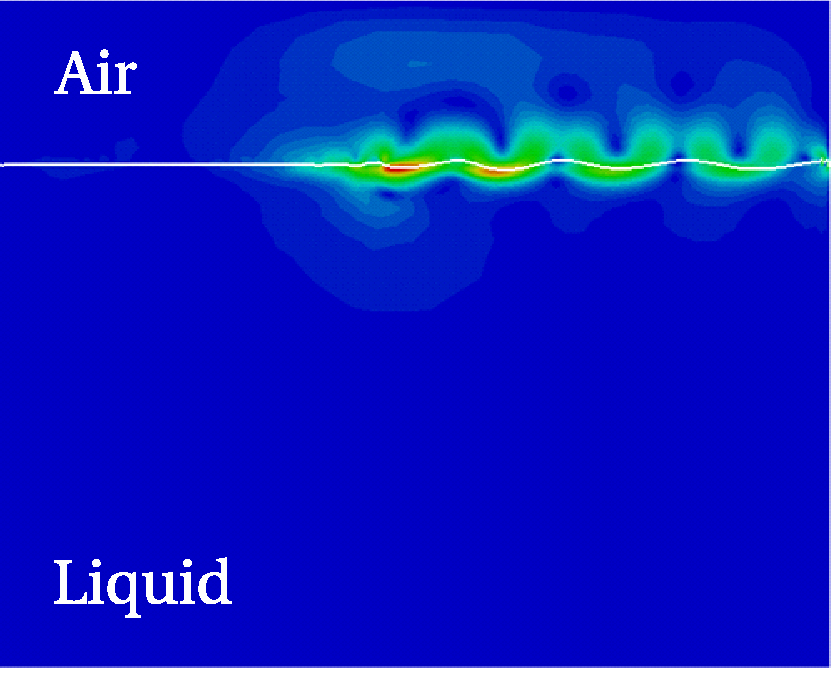
\includegraphics[width=\textwidth]{Chapter4/Graphics/UnstableInterface1.pdf}
	\caption{At a certain time increment (without mesh)}
    \label{fig:UnstableInterface1}
  \end{subfigure}
\qquad
 \begin{subfigure}[t]{0.4\textwidth}
    \centering
	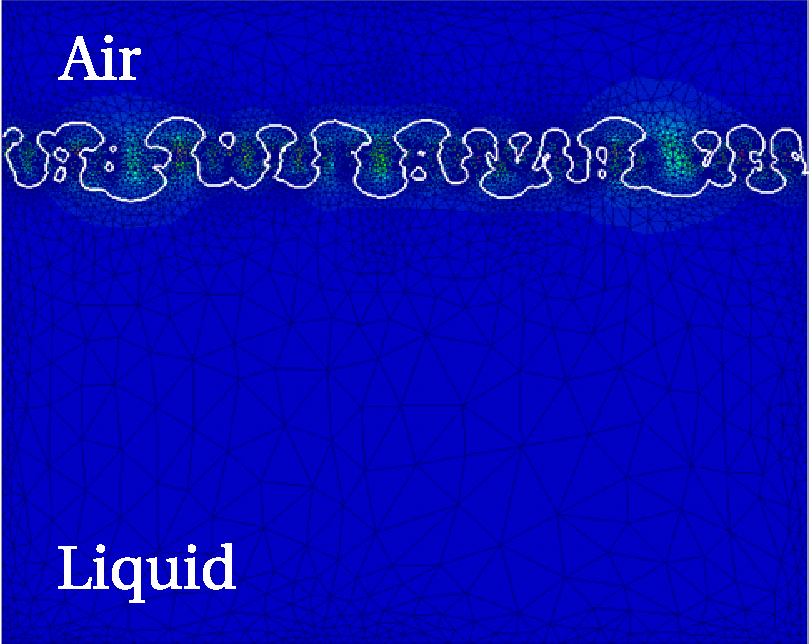
\includegraphics[width=\textwidth]{Chapter4/Graphics/UnstableInterface2.pdf}
	\caption{Another time increment (with mesh)}
    \label{fig:UnstableInterface2}
  \end{subfigure}
\caption{Interface destabilisation under the effect of high properties ratio across the interface.}
\end{figure}
%----------------------
%%---------
\subsubsection{Modified coupling}
In contrast to a classic coupling, here we attempt to modify the velocity field before feeding to the transport solver.
The main motivation for considering this approach is the lack of stability that we observed whenever the mechanical
properties of the fluids were different by several orders of magnitude.
The algorithm should simultaneously fulfil these requirements: 
\begin{itemize}
\itemsep0em
\item support high ratios of fluids density with close viscosities by preserving an non-oscillating interface,
\item maintain a horizontal level at the free surface of the melt,
\item follow shrinking metal surface profile in solidfying regions,
\item satisfy the mass conservation principle, essentially in the metal.
\end{itemize}
We want to process the original transport velocity by imposing a uniform motion (speed and direction) 
at the nodes of the free surface, and at the same time, be able to follow the pipe formation at the 
surface as a result of solidification shrinkage, as shown in \cref{fig:horizontal_liquid_surface}.
%----------------------
\begin{figureth}
% textwidth 
{0.8}
%path 
{Chapter4/Graphics/FreeSurface.pdf}
% caption
{Snapshot of a solidifying ingot by a cooling flux from the side. The profile of the actual surface changes in solid and mushy regions
to adapt the new density while staying perfectly horizontal in the liquid phase.}
% label
\label{fig:horizontal_liquid_surface}
\end{figureth}
%-----------------------------------
%
\comment{How to transport level set using velocity from momentum conservation DIRECTLY or AVERAGED PER ELEMENTS, 
show examples of instability/stability when using false/nominal air properties \\ 
Validation of LS transport: perform test case simulation of buoyancy driven air droplet in water by 2005Nagrath that I also have seen 
in Shyamprasad's masters report). => I didnt notice: what time step $\delta t$ did they use ? }
%
%----------------------
\begin{figureth}
% textwidth 
{0.8}
%path 
{Chapter4/Graphics/AvgTransport/BottomSideCooling.pdf}
% caption
{Treatment of liquid free surface in a) bottom and b) side heat extraction configurations. The dashed line represents the 
initial level of the free liquid surface.}
% label
\label{fig:bottom_side_cooling}
\end{figureth}
%-----------------------------------
The general idea is read the velocity around the interface up to a certain thickness, which may be the same 
thickness as the diffuse interface defined in \cref{sec:heaviside}, then compute a volumetric average
from all the elements in the thickness. This average is then given to the transport solver, which will apply
the same magnitude and direction to transport the interface. However, as we only need the transport velocity
to be uniform within the "100\% liquid" elements, it should not be the case for the other elements that belong 
either to the mushy zone or the solid region, where shrinkage is taking place.
Therefore, depending on the heat extraction configuration, two scenarios are possible. If heat extraction is far from
the interface, i.e. there is not direct contact as in \cref{fig:bottom_side_cooling}a, the surface area remains unchanged at any time, hence all the elements
around the interface are "100\% liquid". This happens when a bottom cooling is applied to the ingot. In contrast, if a side cooling 
is applied as shown in \cref{fig:bottom_side_cooling}b, the surface area of the interface will be reduced over time
as a consequence of the solid front progression. In this case, the average transport velocity should be computed only
from the elements belonging to the free surface. The remaining part of the interface which belongs to partial or full 
solid regions, is transported with Navier-Stokes output, which should be some orders of magnitude less than the velocity
imposed at the free surface, as a result of a decreasing permeability.

%
%--------------------------------
\section{Shrinkage without macrosegregation}
Explain how the flow and heat transfer in the air are not important \\ 
Give the strong form equations to be solved OR simply refer the previous section where the model was defined \\
Initial and boundary conditions for energy and momentum:  Initially we have liquid and air at rest. 
%--
\subsection{Al-7wt\% Si}
Present pseudo 1D case with results + discussion
%--
\subsection{Pb-3wt\% Sn}
Present 2D and 3D case with results + discussion
%--
%--------------------------------
\section{Shrinkage with macrosegregation}
Explain how the flow and heat transfer in the air are not important \\ 
Give the strong form equations to be solved OR simply refer the previous section where the model was defined \\
Initial and boundary conditions for energy and momentum:  Initially we have liquid and air at rest. 
%--
\subsection{Al-7wt\% Si}
Present pseudo 1D case with results + discussion
%--
\subsection{Pb-3wt\% Sn}
Present 2D and 3D case with results + discussion
%--

